\documentclass[]{book}

%These tell TeX which packages to use.
\usepackage{array,epsfig}
\usepackage{amsmath}
\usepackage{amsfonts}
\usepackage{amssymb}
\usepackage{amsxtra}
\usepackage{amsthm}
\usepackage{mathrsfs}
\usepackage{color}
\usepackage{graphicx}
\usepackage{bm}
\usepackage{tikz}
\usepackage{float}
\usepackage{titlesec}

\setcounter{secnumdepth}{4}
%\usepackage{widthof}
\usetikzlibrary{arrows}

%Here I define some theorem styles and shortcut commands for symbols I use often
\theoremstyle{definition}
\newtheorem{defn}{Definition}
\newtheorem{thm}{Theorem}
\newtheorem{cor}{Corollary}
\newtheorem*{rmk}{Remark}
\newtheorem{lem}{Lemma}
\newtheorem*{joke}{Joke}
\newtheorem{ex}{Example}
\newtheorem*{soln}{Solution}
\newtheorem{prop}{Proposition}

\newcommand{\lra}{\longrightarrow}
\newcommand{\ra}{\rightarrow}
\newcommand{\surj}{\twoheadrightarrow}
\newcommand{\graph}{\mathrm{graph}}
\newcommand{\bb}[1]{\mathbb{#1}}
\newcommand{\Z}{\bb{Z}}
\newcommand{\Q}{\bb{Q}}
\newcommand{\R}{\bb{R}}
\newcommand{\C}{\bb{C}}
\newcommand{\N}{\bb{N}}
\newcommand{\M}{\mathbf{M}}
\newcommand{\m}{\mathbf{m}}
\newcommand{\MM}{\mathscr{M}}
\newcommand{\HH}{\mathscr{H}}
\newcommand{\Om}{\Omega}
\newcommand{\Ho}{\in\HH(\Om)}
\newcommand{\bd}{\partial}
\newcommand{\del}{\partial}
\newcommand{\bardel}{\overline\partial}
\newcommand{\textdf}[1]{\textbf{\textsf{#1}}\index{#1}}
\newcommand{\img}{\mathrm{img}}
\newcommand{\ip}[2]{\left\langle{#1},{#2}\right\rangle}
\newcommand{\inter}[1]{\mathrm{int}{#1}}
\newcommand{\exter}[1]{\mathrm{ext}{#1}}
\newcommand{\cl}[1]{\mathrm{cl}{#1}}
\newcommand{\ds}{\displaystyle}
\newcommand{\vol}{\mathrm{vol}}
\newcommand{\cnt}{\mathrm{ct}}
\newcommand{\osc}{\mathrm{osc}}
\newcommand{\LL}{\mathbf{L}}
\newcommand{\x}{\bm{x}}
\newcommand{\UU}{\mathbf{U}}
\newcommand{\support}{\mathrm{support}}
\newcommand{\AND}{\;\wedge\;}
\newcommand{\OR}{\;\vee\;}
\newcommand{\Oset}{\varnothing}
\newcommand{\st}{\ni}
\newcommand{\wh}{\widehat}

%Pagination stuff.
\setlength{\topmargin}{-.3 in}
\setlength{\oddsidemargin}{0in}
\setlength{\evensidemargin}{0in}
\setlength{\textheight}{9.in}
\setlength{\textwidth}{6.5in}
\pagestyle{empty}
\renewcommand{\thesection}{\arabic{section}}



\begin{document}

\begin{center}
{\Large Draft}\\
\textbf{Alireza Abrehforoush}\\ %You should put your name here
Date: 8-17-2022 %You should write the date here.
\end{center}
\vspace{0.2 cm}
%%%%%%%%%%%%%%%%%%%%%%%%%%%%%%%%%%%%%%%%%%%
\section{Synchronous dynamics}
\begin{figure}[H]
    \centering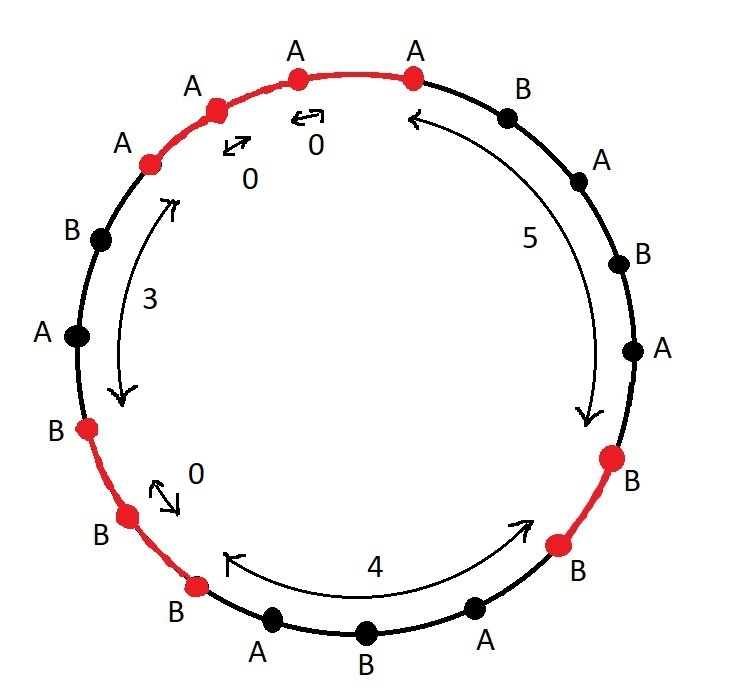
\includegraphics[width=0.4\textwidth]{figures/pic2.jpg}
    \caption{configuration with $\left(c_{1}, c_{2}, c_{3}, c_{4}, c_{5}, c_{6}\right) = \left(5, 4, 0, 3, 0, 0\right)$}
    %\label{fig:mesh2}
\end{figure}
\begin{figure}[H]
    \centering
    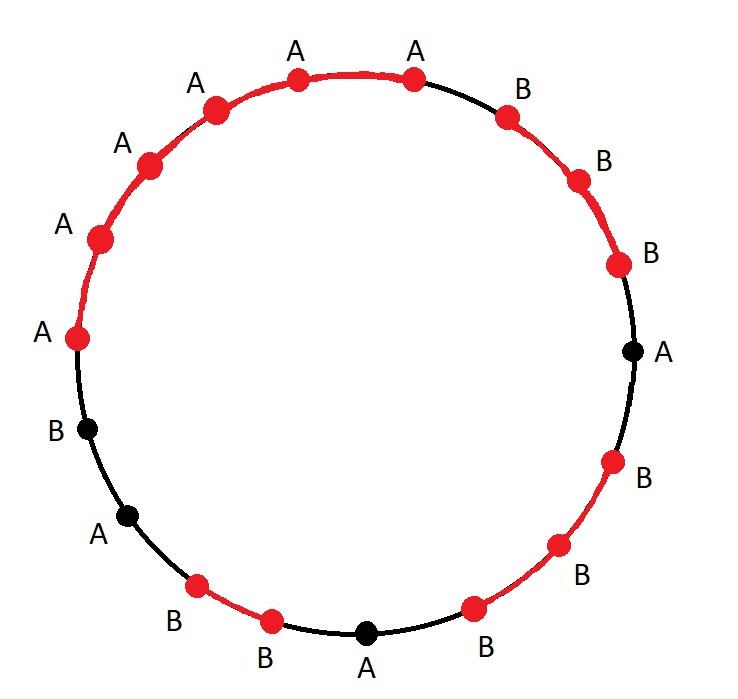
\includegraphics[width=0.4\textwidth]{figures/sync.jpg}
    \caption{configuration with $\left(c_{1}, c_{2}, c_{3}, c_{4}, c_{5}, c_{6}, c_{7}, c_{8}, c_{9}, c_{10}\right) = \left(1, 0, 2, 0, 2, 2, 0, 0, 0, 0\right)$}
    %\label{fig:mesh2}
\end{figure}

Corresponding to all configurations with $i$ red arcs of length one (for simplicity from now on we call it red arcs), we consider a \emph{system} $i^\prime$ in which our random walker is wandering and leaves it after a while. As in synchronous dynamics at each time step, the number of red arcs is either ascending (appearance of red arcs due to activation of all coordinating agents on an arc by at most twice number of current red arcs) or descending (disappearance of any number of red arcs due to activation of the agent adjacent to two red arcs), these systems can be modeled through below directed graphs regarding the parity of number of red arcs of length one at the beginning ($m$):

%graph
\begin{figure}[H]
    \centering
    \begin{tikzpicture}
    \tikzset{vertex/.style = {shape=circle,draw,minimum size=3em}}
    \tikzset{edge/.style = {->,> = latex'}}
    % vertices
    \node[vertex] (a0) at  (0,0) {$0^\prime$};
    
    \node[vertex] (a2) at  (0,-2) {$2^\prime$};
    \node[vertex] (b0) at  (-2,-4) {$0^\prime$};
    \node[vertex] (b4) at  (0,-4) {$4^\prime$};
    \node[vertex] (b6) at  (2,-4) {$6^\prime$};
    \path[->] (a2) edge
    node[above]{} (b0);
    \path[->] (a2) edge
    node[above]{} (b4);
    \path[->] (a2) edge
    node[above]{} (b6);
%%%%%%%%%%%%%%%%%
    \node[vertex] (a4) at  (0,-6) {$4^\prime$};
    \node[vertex] (c0) at  (-5,-8) {$0^\prime$};
    \node[vertex] (c2) at  (-3,-8) {$2^\prime$};
    \node[vertex] (c6) at  (-1,-8) {$6^\prime$};
    \node[vertex] (c8) at  (1,-8) {$8^\prime$};
    \node[vertex] (c10) at  (3,-8) {$10^\prime$};
    \node[vertex] (c12) at  (5,-8) {$12^\prime$};
    \path[->] (a4) edge
    node[above]{} (c0);
    \path[->] (a4) edge
    node[above]{} (c2);
    \path[->] (a4) edge
    node[above]{} (c6);
    \path[->] (a4) edge
    node[above]{} (c8);
    \path[->] (a4) edge
    node[above]{} (c10);
    \path[->] (a4) edge
    node[above]{} (c12);
%%%%%%%%%%%%%%%%%
    \node[vertex] (a6) at  (0,-10) {$6^\prime$};
    \node[vertex] (d0) at  (-8,-12) {$0^\prime$};
    \node[vertex] (d2) at  (-6,-12) {$2^\prime$};
    \node[vertex] (d4) at  (-4,-12) {$4^\prime$};
    \node[vertex] (d8) at  (-2,-12) {$8^\prime$};
    \node[vertex] (d10) at  (0,-12) {$10^\prime$};
    \node[vertex] (d12) at  (2,-12) {$12^\prime$};
    \node[vertex] (d14) at  (4,-12) {$14^\prime$};
    \node[vertex] (d16) at  (6,-12) {$16^\prime$};
    \node[vertex] (d18) at  (8,-12) {$18^\prime$};
    \path[->] (a6) edge
    node[above]{} (d0);
    \path[->] (a6) edge
    node[above]{} (d2);
    \path[->] (a6) edge
    node[above]{} (d4);
    \path[->] (a6) edge
    node[above]{} (d8);
    \path[->] (a6) edge
    node[above]{} (d10);
    \path[->] (a6) edge
    node[above]{} (d12);
    \path[->] (a6) edge
    node[above]{} (d14);
    \path[->] (a6) edge
    node[above]{} (d16);
    \path[->] (a6) edge
    node[above]{} (d18);
%%%%%%%%%%%%%%%%%
    \node[vertex] (a) at  (0,-16) {$n^\prime$};
    \node[vertex] (e0) at  (-6,-18) {$0^\prime$};
    \node[vertex] (e2) at  (-4,-18) {$2^\prime$};
    \node[vertex] (en_2) at  (6,-18) {$(n-2)^\prime$};
    \path[->] (a) edge
    node[above]{} (e0);
    \path[->] (a) edge
    node[above]{} (e2);
    \path[->] (a) edge
    node[above]{} (en_2);
    \path (e2) to node {\dots} (en_2);
    
    
    \path (d10) to node {\vdots} (a);

    \end{tikzpicture}
    \caption{systems starting with at most even number of red arcs of length one ($m$)}
\end{figure}
%graph
and respectively for odd number of red arcs.

We denote the upper bound of stay time of our random walker on expectation in system $i$ and reaching to system $j$ by $T_{i, j}$. So the expected time to reach equilibrium starting from any arbitrary configuration ($T$) would be sum of $T_{i,j}$s.



For computing $T$ we have two following approaches:
\subsection{Using  part 1}

We assume $X_1, X_2, \hdots, X_k$ are the red arcs that disappear in this configuration in next time step (Obviously $X$s must be adjacent pairwise) and $Y_1, Y_2, \hdots, Y_h$  are black arcs that appear in this configuration in next time step (Obviously $Y$s must be the black arcs adjacent to ending red arcs of a consecutive adjacent red arcs)


\subsection{Using recurrence relation}

%%%%%%%%%%%%%%%%%%%%%%%%%%%%%%%%%%%%%%%%%%%
%%%%%%%%%%%%%%%%%%%%%%%%%%%%%%%%%%%%%%%%%%%
%%%%%%%%%%%%%%%%%%%%%%%%%%%%%%%%%%%%%%%%%%%
%%%%%%%%%%%%%%%%%%%%%%%%%%%%%%%%%%%%%%%%%%%
%%%%%%%%%%%%%%%%%%%%%%%%%%%%%%%%%%%%%%%%%%%
%%%%%%%%%%%%%%%%%%%%%%%%%%%%%%%%%%%%%%%%%%%
%%%%%%%%%%%%%%%%%%%%%%%%%%%%%%%%%%%%%%%%%%%
%%%%%%%%%%%%%%%%%%%%%%%%%%%%%%%%%%%%%%%%%%%
\newpage
\begin{center}
Date: 8-24-2022
\end{center}

\subsection{Pure decrease of red arcs}
\begin{figure}[H]
    \centering
    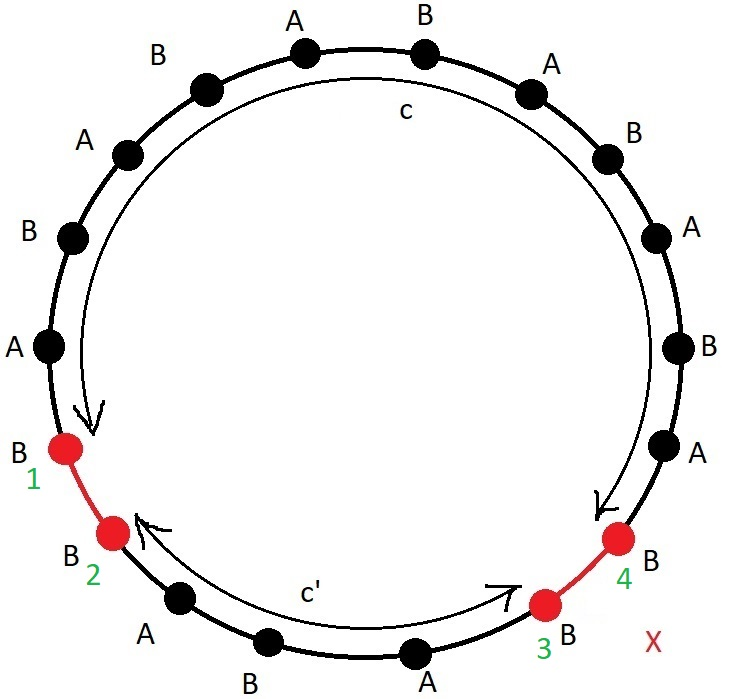
\includegraphics[width=0.4\textwidth]{figures/sync_pure_increase_2.jpg}
    \caption{}
\end{figure}
First of all we try to calculate the expected time to reach equilibrium from a configuration with two red arcs of length 1 (above figure). The recurrence relation is as follows:
\begin{equation}
\begin{split}
    t_c &= \left[2p\left(1-p\right)^3\right] \times \left( t_{c-1}+t_{c+1} \right) \\
    &+ \left[p^2\left(1-p\right)^2\right] \times \left( t_{c-2}+t_{c+2} \right) \\
    &+ \left[1-4p\left(1-p\right)^3-2p^2\left(1-p\right)^2\right] \times t_c \\
    &+ 1,  \quad c = 2,\ldots,n-4
\end{split}
\end{equation}
with following initial conditions:
\begin{equation}
\begin{split}
    t_0 &= \left[ p^2(1-p) \right] \times t_2 \\
    &+ \left[ 2p(1-p)^2 \right] \times t_1 \\
    &+ \left[ 1 -  p^2(1-p) - 3p(1-p)^2 \right] \times t_0 \\
    &+ 1 \\
\end{split}
\end{equation}

\begin{equation}
\begin{split}
    t_1 &= \left[ p^2(1-p)^2 \right] \times t_3 \\
    +& \left[ 2p(1-p)^3 \right] \times t_2 \\
    +& \left[ 1 - 2p^2(1-p)^2 - 4p(1-p)^3 \right] \times t_1 \\ 
    +& \left[ 2p(1-p)^3 \right] \times t_0 \\
    +& 1 \\
\end{split}
\end{equation}
The equations for $n=10$ is as follows:
\begin{equation}
\begin{split}
2t_2+2t_3=2\beta t_0 + (1-\gamma)t_1 + (1+\gamma)t_2 +
(2-2\beta)t_3 +
t_4 +
5 \\
2\beta
\end{split}
\end{equation}
Solution of $n=10$ is as follows:
\begin{equation}
\begin{split}
    t_0 &= -\frac{2\,p^5+7\,p^4-72\,p^3+44\,p^2+160\,p-144}{16\,p^2\,\left(p^2-2\right)\,{\left(p-1\right)}^3} \\ \\
    t_1 &= -\frac{2\,p-9}{2\,p^2\,{\left(p-1\right)}^2} \\ \\
    t_2 &= -\frac{-2\,p^5+13\,p^4-90\,p^3+84\,p^2+136\,p-144}{16\,p^2\,\left(p^2-2\right)\,{\left(p-1\right)}^3} \\ \\
    t_3 &= -\frac{2\,p^3-25\,p^2+8\,p+36}{4\,p^2\,\left(p^2-2\right)\,{\left(p-1\right)}^2} \\ \\
    t_4 &= -\frac{2\,p^5+7\,p^4-120\,p^3+148\,p^2+104\,p-144}{16\,p^2\,\left(p^2-2\right)\,{\left(p-1\right)}^3} \\ \\
    t_5 &= -\frac{2\,p^3-25\,p^2+8\,p+36}{4\,p^2\,\left(p^2-2\right)\,{\left(p-1\right)}^2} \\ \\
    t_6 &= -\frac{-2\,p^5+13\,p^4-90\,p^3+84\,p^2+136\,p-144}{16\,p^2\,\left(p^2-2\right)\,{\left(p-1\right)}^3} \\ \\
    t_7 &= -\frac{2\,p-9}{2\,p^2\,{\left(p-1\right)}^2} \\ \\
    t_8 &= -\frac{2\,p^5+7\,p^4-72\,p^3+44\,p^2+160\,p-144}{16\,p^2\,\left(p^2-2\right)\,{\left(p-1\right)}^3} \\ \\
\end{split}
\end{equation}
We write equations (1), (2), and (3) as following matrix operation:
\begin{equation}
\begin{pmatrix}
\alpha & \alpha & \beta & \beta & \gamma & 1
\end{pmatrix}
\begin{pmatrix}
\lambda t_2 & \eta   t_3 & t_1 & t_2 & t_3 & \ldots & t_{n-5} & t_2  & t_1 \\
 \theta t_1 &        t_2 & t_3 & t_4 & t_5 & \ldots & t_{n-3} & t_4  & t_3 \\
 \delta t_0 & \omega t_1 & t_0 & t_1 & t_2 & \ldots & t_{n-6} & t_1  & t_0 \\
          0 & \sigma t_0 & t_4 & t_5 & t_6 & \ldots & t_{n-2} & t_5  & t_4 \\
          0 &          0 & t_2 & t_3 & t_4 & \ldots & t_{n-4} & t_3  & t_2 \\
          1 &          1 &   1 &   1 &   1 & \ldots &       1 &   1  &   1
\end{pmatrix}_{6\times n-1}=
\begin{pmatrix}
t_0 & t_1 & t_2 & t_3 & t_4 & \ldots & t_{n-4} & t_{n-3} & t_{n-2}
\end{pmatrix}
\end{equation}
\begin{equation}
\begin{split}
    \alpha &= 2p(1-p)^3 \\
    \beta &= p^2(1-p)^2 \\
    \gamma &= 1 - 4p(1-p)^3 - 2p^2(1-p)^2 \\
    \lambda &= \frac{p^2(1-p)}{\alpha} \\
    \theta &= \frac{2p(1-p)^2}{\alpha} \\
    \delta &= \frac{1 -  p^2(1-p) - 3p(1-p)^2}{\beta} \\
    \eta &=  \frac{p^2(1-p)^2}{\alpha} \\
    \omega &= \frac{1 -  2p^2(1-p)^2 - 4p(1-p)^3}{\beta} \\
    \sigma &= \frac{\alpha}{\beta}
\end{split}
\end{equation}
% \begin{equation}
% \begin{split}
% \sum_{i=4}^{n-2}t_i=\frac{2p-2}{p}\sum_{i=3}^{n-3}t_i
% +\frac{4-2p}{p}\sum_{i=2}^{n-4}t_i
% +\frac{2p-2}{p}\sum_{i=1}^{n-5}t_i
% -\sum_{i=0}^{n-6}t_i
% +\frac{-(n-1)}{p^2(1-p)^2} \\
% \Rightarrow
% 2t_0+\frac{4-2p}{p}t_1-\frac{4-2p}{p}t_2-2t_3=\frac{-(n-1)}{p^2(1-p)^2}
% \end{split}
% \end{equation}
% Recurrence relation is standard form:
% \begin{equation}
% \begin{split}
%     t_{c+2} &= \frac{2p-2}{p}t_{c+1} \\
%     +& \frac{4-2p}{p}t_{c} \\
%     +& \frac{2p-2}{p}t_{c-1} \\
%     -& t_{c-2} \\
%     -& \frac{1}{p^2(1-p)^2}
% \end{split}
% \end{equation}
% and following characteristic function:
% \begin{equation}
% \begin{split}
%     r^4 - \frac{2p-2}{p}r^3
%     - \frac{4-2p}{p}r^2
%     - \frac{2p-2}{p}r
%     + 1 = 0
% \end{split}
% \end{equation}
% Online solver provided following general solution solution (without considering initial conditions)
% \begin{figure}[H]
%     \centering
%     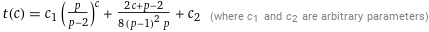
\includegraphics[width=1\textwidth]{figures/2r.jpg}
%     \caption{}
%     %\label{fig:mesh2}
% \end{figure}





\subsubsection{Pure increase of red arcs}
\begin{figure}[H]
    \centering
    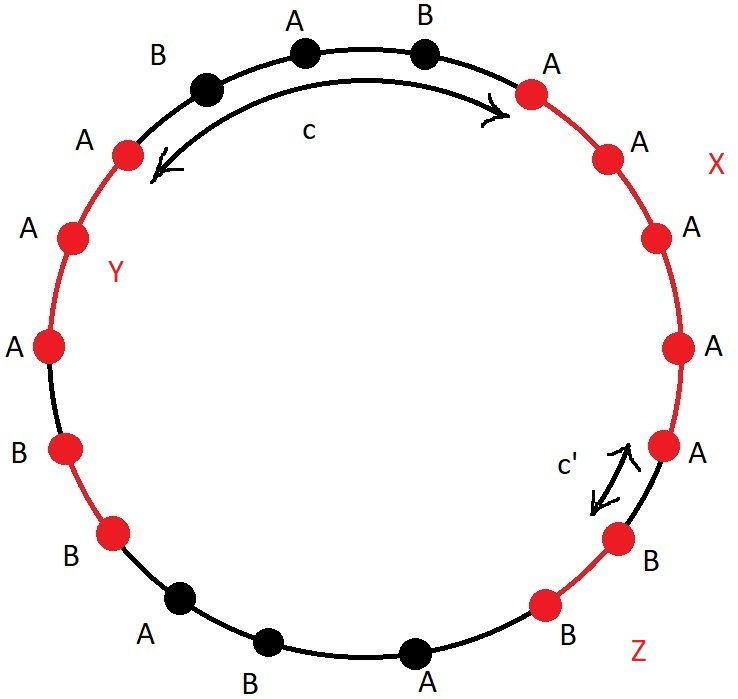
\includegraphics[width=0.4\textwidth]{figures/sync_pure_increase_general.jpg}
    \caption{}
    %\label{fig:mesh2}
\end{figure}

To analyze this configuration, we begin by the case that there is only one red arc of length $k$ that causes to reach system $(m+2)^\prime$ (denoted by $X$). If we are able to show that this cannot happen in less than exponential time for specific values of $p$, then we can conclude that the configuration can reach equilibrium in polynomial time.

At first, we try to solve the basic cases. In following configuration the expected time to reach system $3^\prime$ (only odd number of agents) $s$. 
\begin{figure}[H]
    \centering
    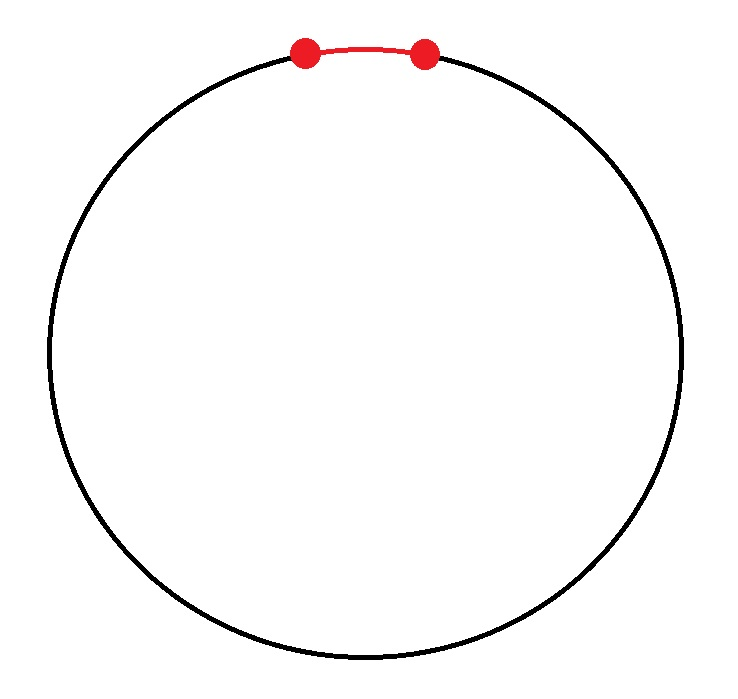
\includegraphics[width=0.4\textwidth]{figures/sync_pure_increase_1.jpg}
    \caption{}
    %\label{fig:mesh2}
\end{figure}
We can calculate $s$ as follows:
\begin{equation}
\begin{split}
    &s = p^2 \times 0 + \left( 1 - p^2 \right)\times s + 1 \\
    \Rightarrow &s = \frac{1}{p^2}
\end{split}
\end{equation}

\begin{figure}[H]
    \centering
    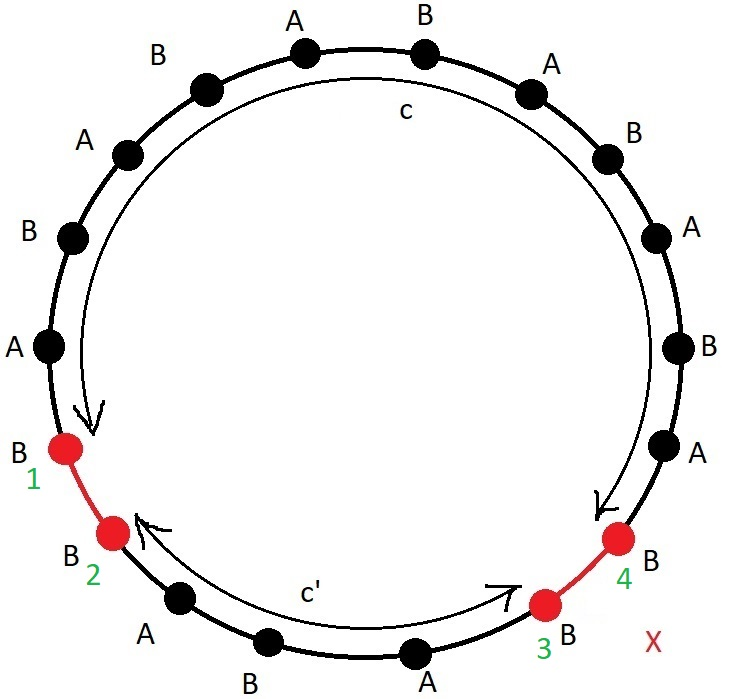
\includegraphics[width=0.4\textwidth]{figures/sync_pure_increase_2.jpg}
    \caption{}
    %\label{fig:mesh2}
\end{figure}

\subsection{Simultaneous decrease and increase of red arcs}
%%%%%%%%%%%%%%%%%%%%%%%%%%%%%%%%%%%%
%%%%%%%%%%%%%%%%%%%%%%%%%%%%%%%%%%%%
%%%%%%%%%%%%%%%%%%%%%%%%%%%%%%%%%%%%
%%%%%%%%%%%%%%%%%%%%%%%%%%%%%%%%%%%%
%%%%%%%%%%%%%%%%%%%%%%%%%%%%%%%%%%%%
%%%%%%%%%%%%%%%%%%%%%%%%%%%%%%%%%%%%
%%%%%%%%%%%%%%%%%%%%%%%%%%%%%%%%%%%%
%%%%%%%%%%%%%%%%%%%%%%%%%%%%%%%%%%%%
\newpage
\begin{center}
Date: 8-31-2022
\end{center}

\subsection{Pure increase of red arcs}
\subsubsection{Base case (with two arcs of size 1)}
\begin{figure}[H]
    \centering
    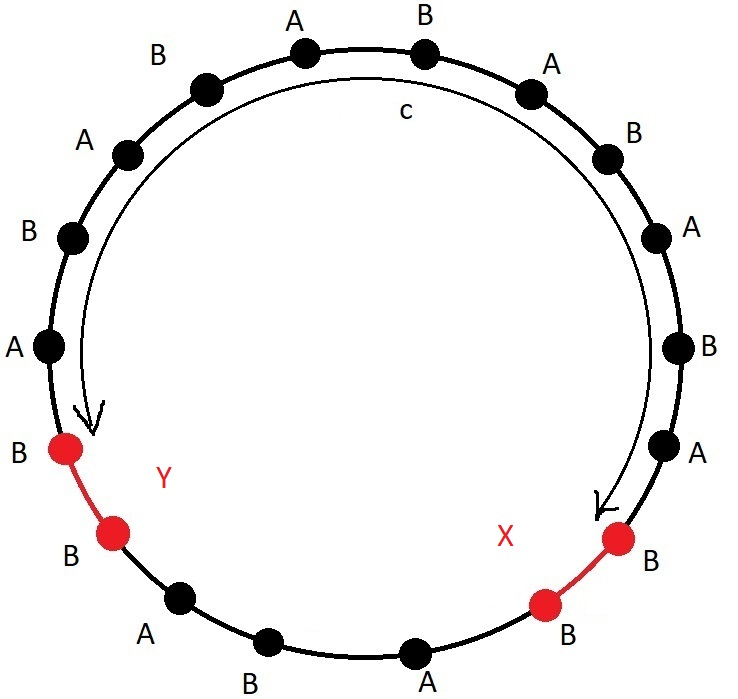
\includegraphics[width=0.4\textwidth]{figures/sync_pure_increase_3.jpg}
    \caption{}
\end{figure}

In the above configuration, we consider that $X$ is the first and only red arc through which the transition from system $2^\prime$ to system $4^\prime$ happens. Thus, before the transition $X$ is just wandering in black region. Let $s_c$ be the time required for the transition of $X$ with respect to distance $c$ from $Y$. The changes in $s_c$ are governed by the following recurrence relation:
\begin{equation}
\begin{split}
    s_c 
    =& \left[ \left( 1-p \right) ^ 4 + 2p^2 \left( 1-p \right)^2 \right]\times s_c \\
    &+\left[ 2p \left( 1-p \right) ^ 3 \right]\times \left( s_{c-1} + s_{c+1} \right) \\
    &+\left[ p^2\left( 1-p \right)^2 \right]\times \left( s_{c-2} + s_{c+2} \right) \\
    &+1, \quad c = 2,\ldots,n-4,
\end{split}
\end{equation}
and following initial conditions:
\begin{equation}
\begin{split}
    s_0 =s_{n-2} 
    =&\left[ \left( 1-p \right)^3 + 2p^2\left( 1-p \right) \right]\times s_0 \\
    &+\left[ 2p\left( 1-p \right)^2 \right]\times s_1 \\
    &+\left[p^2\left( 1-p \right) \right]\times s_2 \\
    &+1
\end{split}
\end{equation}
% Thus, 
% \begin{equation}
% \begin{split}
% s_{c+2}
% =&
% -\frac{2\left( 1-p \right)}{p}\times s_{c+1} \\
% &+\frac{1-\left( 1-p \right) ^ 4 - 2p^2 \left( 1-p \right) ^2}{p^2 \left( 1-p \right)^2} \times s_c \\
% &-\frac{2\left( 1-p \right)}{p}\times s_{c-1} \\
% &-s_{c-2} \\
% &-\frac{1}{p^2 \left( 1-p \right)^2}
% \end{split}
% \end{equation}

Online solver suggests the following closed form for the above recurrence relation (without considering initial conditions):
\begin{figure}[H]
    \centering
    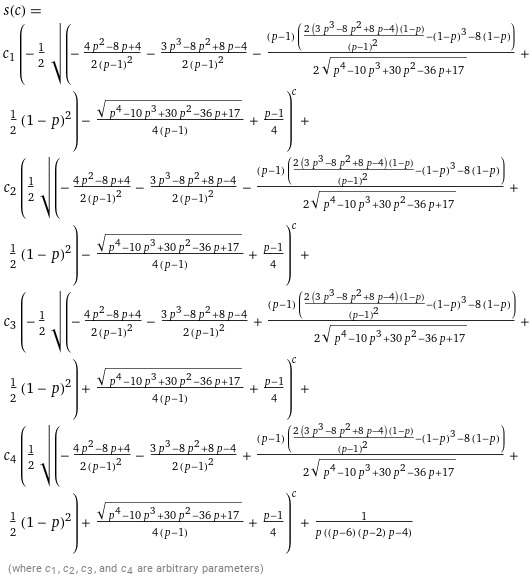
\includegraphics[width=1\textwidth]{figures/equation_1.jpg}
    \caption{}
\end{figure}
And for some specific values of $p$ we have following equations:
\begin{figure}[H]
    \centering
    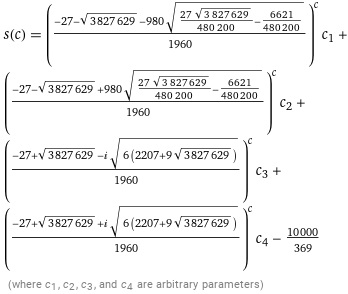
\includegraphics[width=1\textwidth]{figures/equation_2.jpg}
    \caption{for $p=0.2$}
\end{figure}
\begin{figure}[H]
    \centering
    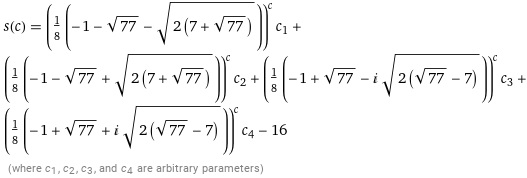
\includegraphics[width=1\textwidth]{figures/equation_3.jpg}
    \caption{for $p=0.5$}
\end{figure}
\begin{figure}[H]
    \centering
    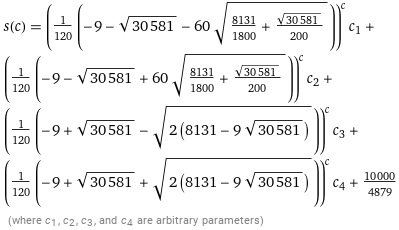
\includegraphics[width=1\textwidth]{figures/equation_4.jpg}
    \caption{for $p=0.7$}
\end{figure}

\subsubsection{Base case ($X$ with arbitrary length)}
\begin{figure}[H]
    \centering
    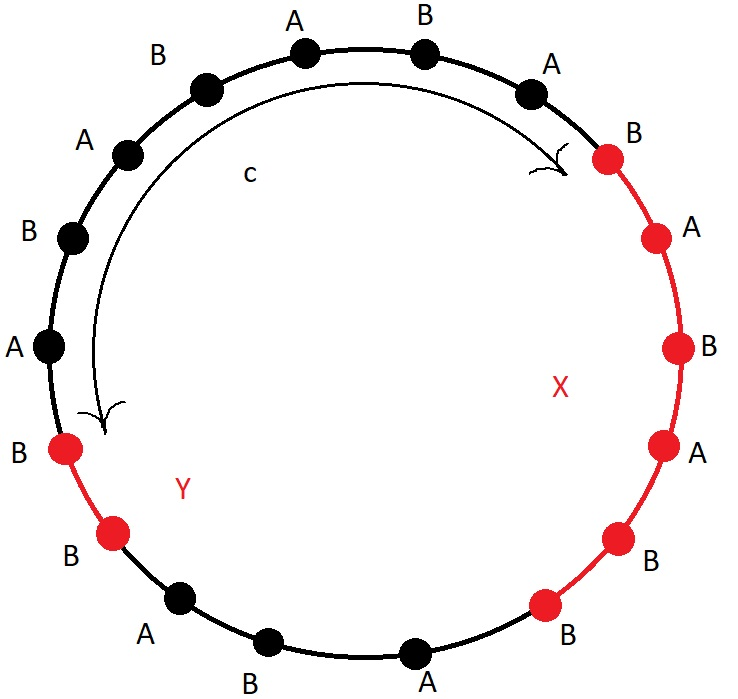
\includegraphics[width=0.4\textwidth]{figures/Sync_base_general.jpg}
    \caption{}
\end{figure}
Let $X$ of length $k$ be the first and only red arc  through which the transition from system $2^\prime$ to system $4^\prime$ happens.
As decomposition of $X$ will decelerate the transition, by assuming that $X$ can only wander in black region (no decomposition occurs before the transition), we can calculate a lower bound for $s_c$. The changes in $s_c$ are governed by the following recurrence relation:
\begin{equation}
\begin{split}
    s_c 
    =& \left[ \left( 1-p \right) ^ {k+1} \left( 1-p \right) ^ 2 + 2p^k \left( 1-p \right)p \left( 1-p \right) \right]\times s_c \\
    &+\left[ \left( 1-p \right) ^ {k+1} p \left( 1-p \right) + p^k \left( 1-p \right)\left( 1-p \right) ^ 2 \right]\times \left( s_{c-1} + s_{c+1} \right) \\
    &+\left[ p^k \left( 1-p \right)p \left( 1-p \right) \right]\times \left( s_{c-2} + s_{c+2} \right) \\
    &+1, \quad c = 2,\ldots,n-k-2,
\end{split}
\end{equation}
and following initial conditions:
\begin{equation}
\begin{split}
    s_0=s_{n-k-2} 
    =&\left[ \left( 1-p \right)^{k+1}\left( 1-p \right) + 2p^{k+1}\left( 1-p \right) \right]\times s_0 \\
    &+\left[ p^{k+1}\left( 1-p \right) + \left( 1-p \right)^{k+1}p \right]\times s_1 \\
    &+\left[2p^k p\left( 1-p \right) \right]\times s_2 \\
    &+1
\end{split}
\end{equation}


And the suggested closed form for the above recurrence relation by online solver is:
%%%%%%%%%%%%%%%%%%%%%%%%%%%%%%%%%%%%
%%%%%%%%%%%%%%%%%%%%%%%%%%%%%%%%%%%%
%%%%%%%%%%%%%%%%%%%%%%%%%%%%%%%%%%%%
%%%%%%%%%%%%%%%%%%%%%%%%%%%%%%%%%%%%
%%%%%%%%%%%%%%%%%%%%%%%%%%%%%%%%%%%%
%%%%%%%%%%%%%%%%%%%%%%%%%%%%%%%%%%%%
%%%%%%%%%%%%%%%%%%%%%%%%%%%%%%%%%%%%
%%%%%%%%%%%%%%%%%%%%%%%%%%%%%%%%%%%%
\newpage
\begin{center}
Date: 9-7-2022
\end{center}


\subsection{Calculating the expected time for each transition between systems}
By \emph{system} we mean a set of configurations having red arcs of same length with respect to their circular order of appearance. We denote a system by shift invariant ordered $k$ tuples $\left( c_1, c_2, \hdots, c_k\right)$ that $c_i$s are the length of red arcs. For example, all configurations below belong to the system $\left( 1, 1 \right)$:
\begin{figure}[H]
    \centering
    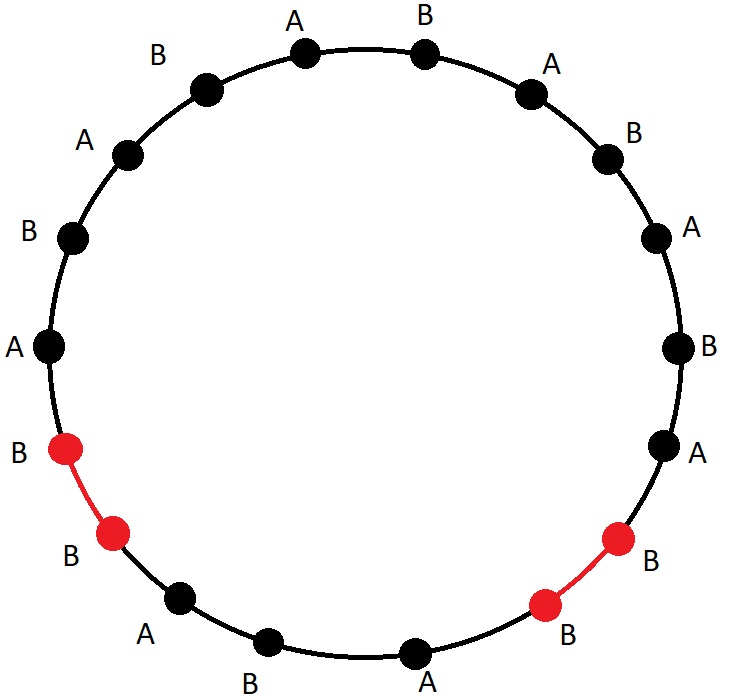
\includegraphics[width=0.4\textwidth]{figures/s1.jpg}
    \caption{}
\end{figure}
\begin{figure}[H]
    \centering
    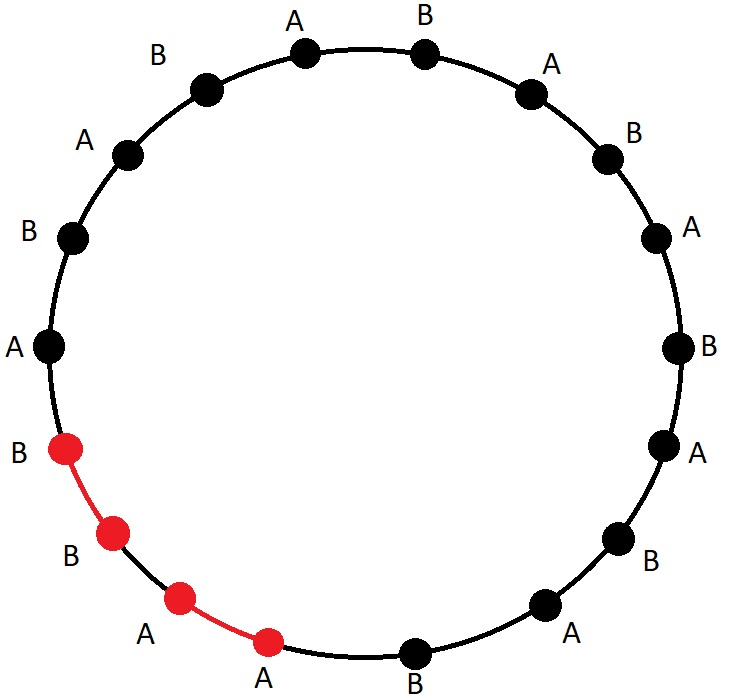
\includegraphics[width=0.4\textwidth]{figures/s2.jpg}
    \caption{}
\end{figure}
Possible transitions for system $\left( 1, 1 \right)$ are shown in following graph:
%graph
\begin{figure}[H]
    \centering
    \begin{tikzpicture}
    \tikzset{vertex/.style = {shape=circle,draw,minimum size=3em}}
    \tikzset{edge/.style = {->,> = latex'}}
    % vertices
    
    \node[vertex] (a2) at  (0,-2) {$\left(1, 1\right)^\prime$};
    \node[vertex] (b0) at  (-2,-4) {$\left(1, 3\right)^\prime$};
    \node[vertex] (b4) at  (0,-4) {$\left(2\right)^\prime$};
    \node[vertex] (b6) at  (2,-4) {$\left(3, 3\right)^\prime$};
    \path[->] (a2) edge
    node[above]{} (b0);
    \path[->] (a2) edge
    node[above]{} (b4);
    \path[->] (a2) edge
    node[above]{} (b6);


    \end{tikzpicture}
    \caption{systems starting with at most even number of red arcs of length one ($m$)}
\end{figure}
%graph

%%%%%%%%%%%%%%%%%%%%%%%%%%%%%%%%%%%%
%%%%%%%%%%%%%%%%%%%%%%%%%%%%%%%%%%%%
%%%%%%%%%%%%%%%%%%%%%%%%%%%%%%%%%%%%
%%%%%%%%%%%%%%%%%%%%%%%%%%%%%%%%%%%%
%%%%%%%%%%%%%%%%%%%%%%%%%%%%%%%%%%%%
%%%%%%%%%%%%%%%%%%%%%%%%%%%%%%%%%%%%
%%%%%%%%%%%%%%%%%%%%%%%%%%%%%%%%%%%%
%%%%%%%%%%%%%%%%%%%%%%%%%%%%%%%%%%%%
\newpage
\begin{center}
Date: 9-15-2022
\end{center}

\subsection{Upper bound for the recurrence relation}
\begin{equation}
\begin{split}
    t_c &= \left[2p\left(1-p\right)^3\right] \times \left( t_{c-1}+t_{c+1} \right) \\
    &+ \left[p^2\left(1-p\right)^2\right] \times \left( t_{c-2}+t_{c+2} \right) \\
    &+ \left[1-4p\left(1-p\right)^3-2p^2\left(1-p\right)^2\right] \times t_c \\
    &+ 1,  \quad c = 2,\ldots,n-4
\end{split}
\end{equation}
% Using the inequality $\left( 1 - p \right) \le e ^ {-p}$ we have:
% \begin{equation}
% \begin{split}
%     t_c &\le \frac{\left[2p e^{-3p}\right] \times \left( t_{c-1}+t_{c+1} \right) + \left[p^2 e^{-2p}\right] \times \left( t_{c-2}+t_{c+2} \right) + 1}{\left[4p\left(1-p\right)^3+2p^2\left(1-p\right)^2\right]} \\
%     &\le 
% \end{split}
% \end{equation}
Online solver suggests following closed form for the simplified form of our recurrence relation \\ ($t_c = x\left( t_{c-1} + t_{c+1} + t_{c-2} + t_{c+2} \right) + y$):
\begin{figure}[H]
    \centering
    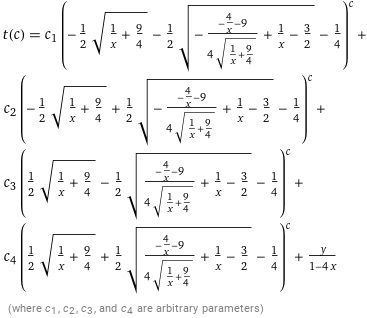
\includegraphics[width=0.7\textwidth]{figures/lower_bound.jpg}
    \caption{}
    %\label{fig:mesh2}
\end{figure}
We try to plot the abstract of each bases of the above exponential expressions (shifted down by 2).
\begin{equation}
\begin{split}
    y_1 &=\left| -\sqrt{\frac{1}{x}+\frac{9}{4}} - \sqrt{-\frac{-\frac{4}{x}-9}{4\sqrt{\frac{1}{x}+\frac{9}{4}}}+\frac{1}{x}-\frac{3}{2}} - \frac{1}{2} \right|-2 \\
    y_2 &=\left| -\sqrt{\frac{1}{x}+\frac{9}{4}} + \sqrt{-\frac{-\frac{4}{x}-9}{4\sqrt{\frac{1}{x}+\frac{9}{4}}}+\frac{1}{x}-\frac{3}{2}} - \frac{1}{2} \right|-2 \\
    y_3 &=\left| \sqrt{\frac{1}{x}+\frac{9}{4}} - \sqrt{\frac{-\frac{4}{x}-9}{4\sqrt{\frac{1}{x}+\frac{9}{4}}}+\frac{1}{x}-\frac{3}{2}} - \frac{1}{2} \right|-2 \\
    y_4 &=\left| \sqrt{\frac{1}{x}+\frac{9}{4}} + \sqrt{\frac{-\frac{4}{x}-9}{4\sqrt{\frac{1}{x}+\frac{9}{4}}}+\frac{1}{x}-\frac{3}{2}} - \frac{1}{2} \right|-2
\end{split}
\end{equation}
\begin{figure}[H]
    \centering
    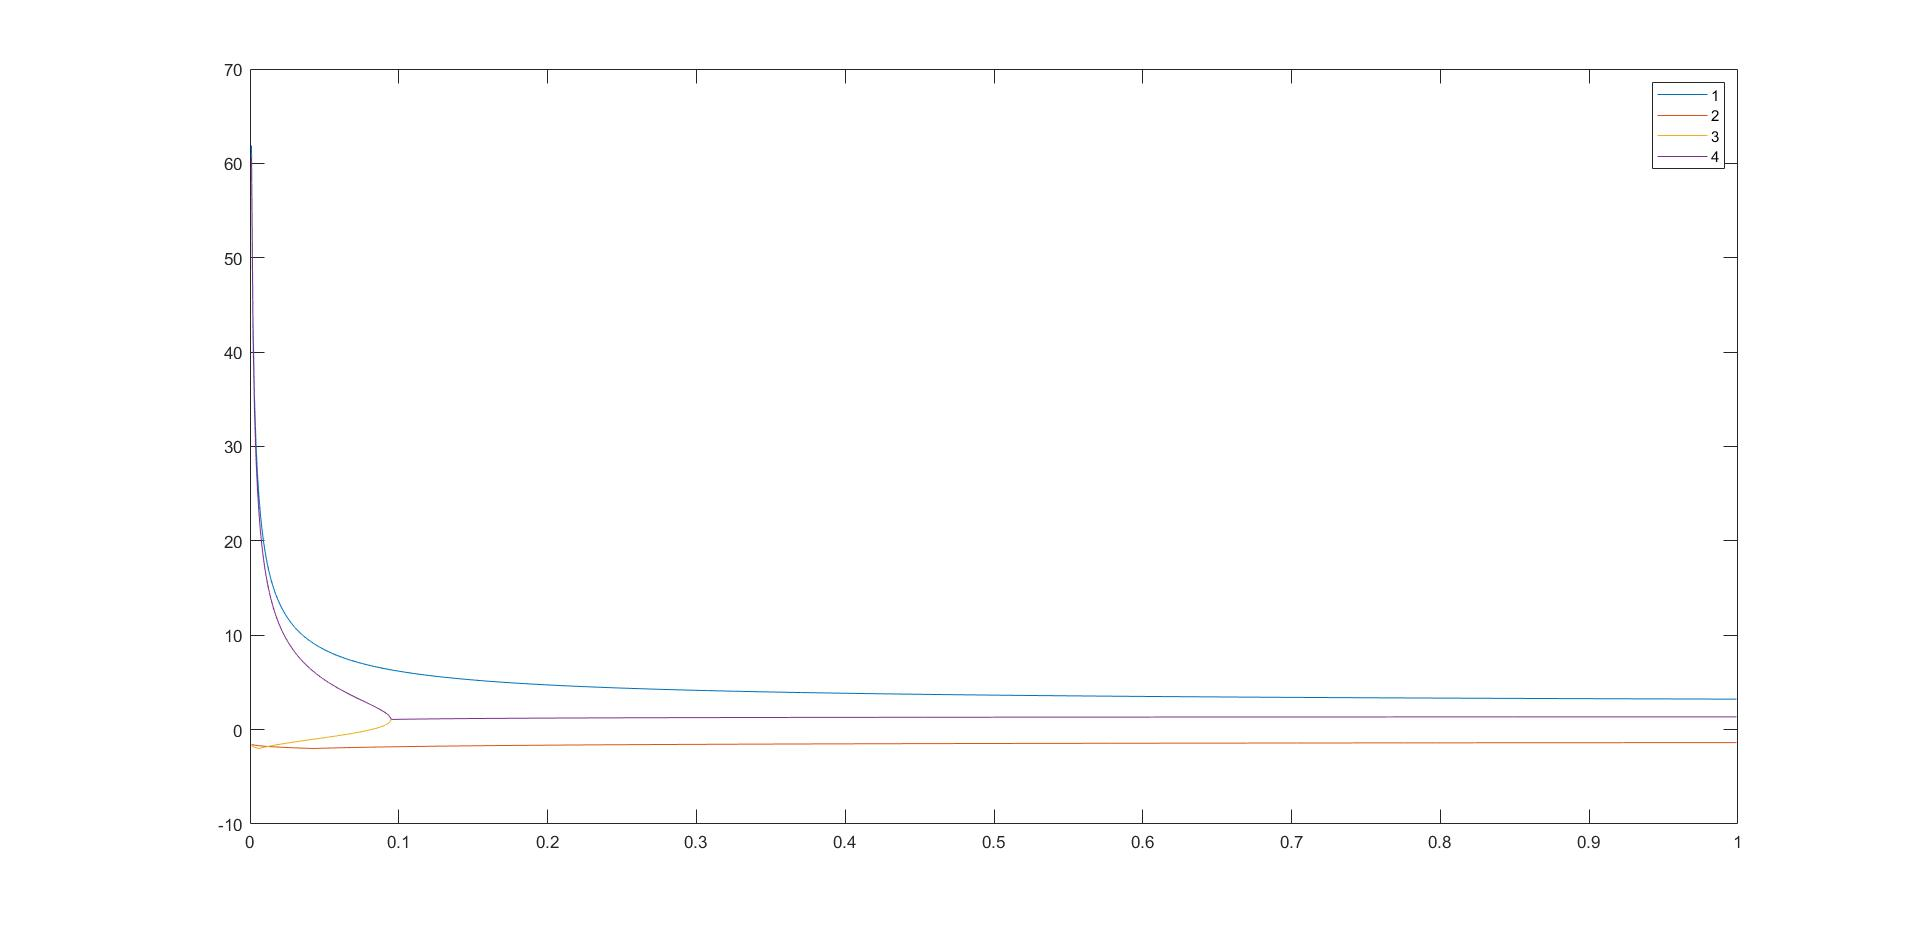
\includegraphics[width=1\textwidth]{figures/matfig1.jpg}
    \caption{}
    %\label{fig:mesh2}
\end{figure}
\begin{figure}[H]
    \centering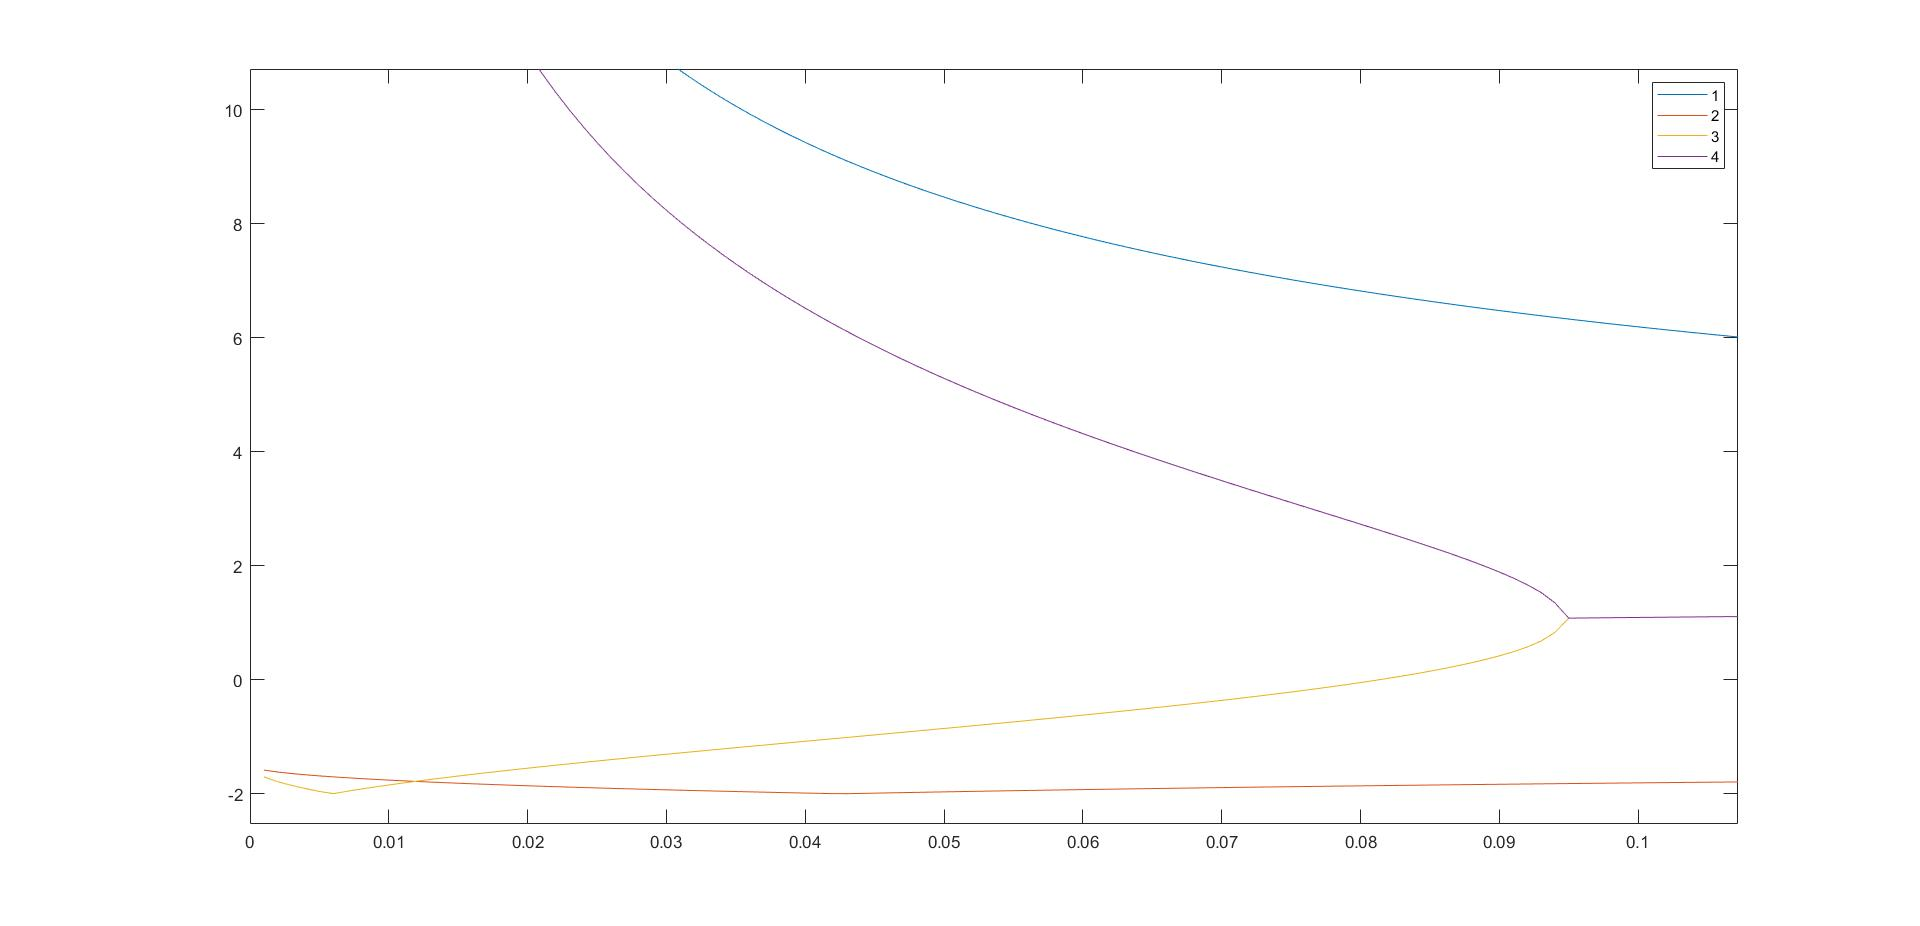
\includegraphics[width=1\textwidth]{figures/matfig2.jpg}
    \caption{}
    %\label{fig:mesh2}
\end{figure}

For $p \ge 1-p$ we can reach following lower bound:
\begin{equation}
\begin{split}
    t_c & \ge \frac{\left[ 1-p \right]^4 \times \left( t_{c-1} + t_{c+1} + t_{c-2} + t_{c+2} \right) + 1}{6p^4}
\end{split}
\end{equation}

\subsection{Unit transitions}
Any transition can be modeled as a combination of following unit transitions:
\subsubsection{Decomposition of a red arc of length $k$ to two red arcs of length $k_1$ and $k_2$ ($k_1 + k_2 = k$)}
\begin{figure}[H]
    \centering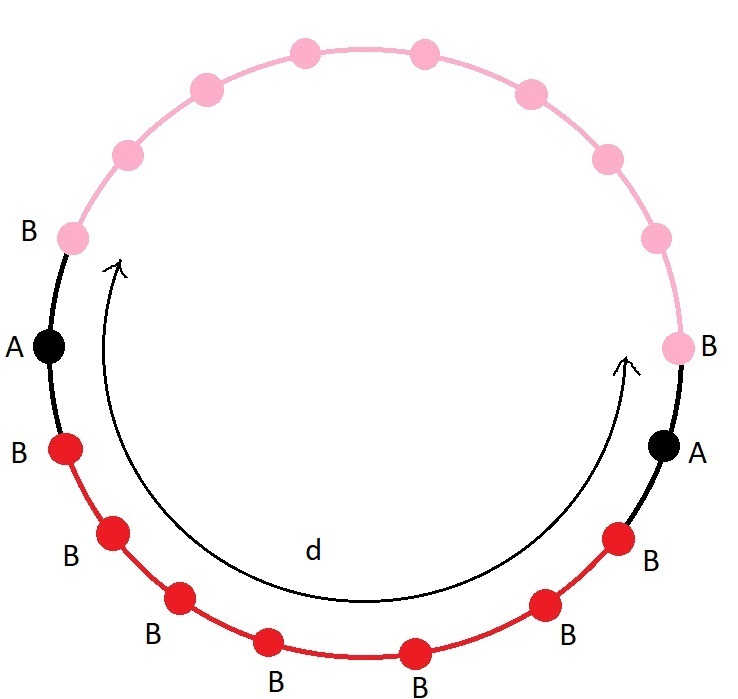
\includegraphics[width=0.4\textwidth]{figures/arc decomposition.jpg}
    \caption{}
    %\label{fig:mesh2}
\end{figure}
In any arbitrary configuration, transition can occur through decomposition of a red arc $X$ of length $k$ which is floating in a black region of length $d$ (i.e. the red arc in above figure) to two red arcs of length $k_1$ and $k_2$. The expected time to reach this system ($t_c$) is calculated as follows:
\begin{equation}
\begin{split}
    t_c &= \left[ p^k\left( 1-p \right) + p^{k_1}\left(1-p\right)^{k-k_1+1} + p^{k_2}\left(1-p\right)^{k-k_2+1} \right] \times 0 \\
    &+ \left[ p^k\left( 1-p \right) \right] \times t_{c-1} \\
    &+ \left[ p^k\left( 1-p \right) \right] \times t_{c+1} \\
    &+ \left[1 - 3p^k\left( 1-p \right) - p^{k_1}\left(1-p\right)^{k-k_1+1} - p^{k_2}\left(1-p\right)^{k-k_2+1} \right] \times t_c \\
    &+ 1, \quad c \in \left\{2, 3, \hdots, d-k-2 \right\}
\end{split}
\end{equation}
with following initial conditions:
\begin{equation}
\begin{split}
    t_1 &= p^k\left( 1-p \right) \times t_2 + \left( 1-p^k\left( 1-p \right) \right) \times t_1 + 1 \\
    t_{d-k-1} &= t_1
\end{split}
\end{equation}

\subsubsection{Decomposition of a red arc of length $k$ to two red arcs of length $k_1$ and $k_2$ ($k_1 + k_2 = k - 2$)}
\begin{figure}[H]
    \centering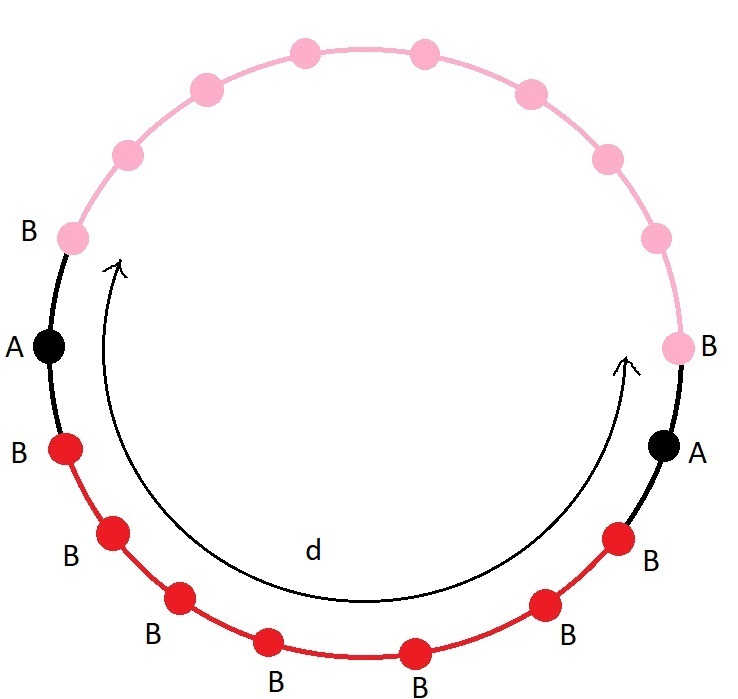
\includegraphics[width=0.4\textwidth]{figures/arc decomposition.jpg}
    \caption{}
    %\label{fig:mesh2}
\end{figure}
In any arbitrary configuration, transition can occur through decomposition of a red arc of length $k$ which is floating in a black region of length $d$ (i.e. the red arc in above figure) to two red arcs of length $k_1$ and $k_2$. The expected time to reach this system ($t_c$) is calculated as follows:
\begin{equation}
\begin{split}
    t_c &= \left[ p^k\left( 1-p \right) \right] \times 0 \\
    &+ \left[ p^k\left( 1-p \right) \right] \times t_{c-1} \\
    &+ \left[ p^k\left( 1-p \right) \right] \times t_{c+1} \\
    &+ \left[1 - 3p^k\left( 1-p \right) \right] \times t_c \\
    &+ 1, \quad c \in \left\{2, 3, \hdots, d-k-2 \right\}
\end{split}
\end{equation}
with following initial conditions:
\begin{equation}
\begin{split}
    t_1 &= p^k\left( 1-p \right) \times t_2 + \left( 1-p^k\left( 1-p \right) \right) \times t_1 + 1 \\
    t_{d-k-1} &= t_1
\end{split}
\end{equation}

\subsubsection{Sticking of two red arcs of lengths $k_1$ and $k_2$ respectively floating in a black region of length $d$ without producing any red arc of length one }
\begin{figure}[H]
    \centering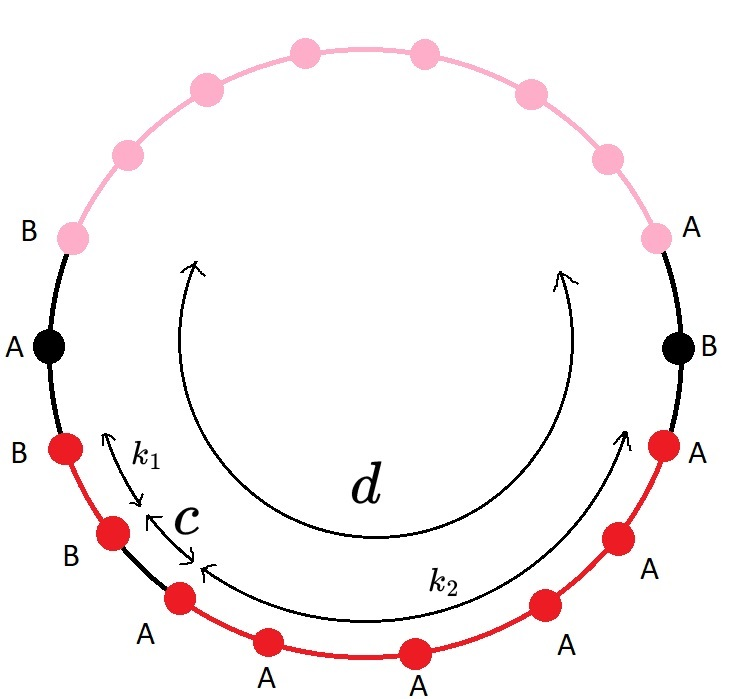
\includegraphics[width=0.4\textwidth]{figures/arcs sticking.jpg}
    \caption{}
    %\label{fig:mesh2}
\end{figure}

\begin{equation}
\begin{split}
    t_c &= \left[p^{k_1}\left( 1-p \right)^{k_2+2} + p^{k_2}\left( 1-p \right)^{k_1+2} \right] \times \left( t_{c-1} + t_{c+1} \right) \\
    &+ \left[ p^{k_1+k_2}\left( 1-p \right)^2 \right] \times \left( t_{c-2}+t_{c+2} \right) \\
    &+ \left[ 1 - 2p^{k_1}\left( 1-p \right)^{k_2+2} - 2p^{k_2}\left( 1-p \right)^{k_1+2} - 2p^{k_1+k_2}\left( 1-p \right)^2 \right] \times t_c \\
    &+ 1, \quad c \in \left\{ 3, 4, \hdots, d - k_1 - k_2 \right\}
\end{split}
\end{equation}
and following initial conditions:
\begin{equation}
\begin{split}
    t_0 &= 0 \\
    t_1 &= \left[p^{k_1}\left( 1-p \right)^{k_2+2} + p^{k_2}\left( 1-p \right)^{k_1+2} \right] \times \left( t_0 + t_2 \right) \\
    &+ \left[ p^{k_1+k_2}\left( 1-p \right)^2 \right] \times t_3 \\
    &+ \left[ 1 - 2p^{k_1}\left( 1-p \right)^{k_2+2} - 2p^{k_2}\left( 1-p \right)^{k_1+2} - p^{k_1+k_2}\left( 1-p \right)^2 \right] \times t_1 \\
    &+ 1
\end{split}
\end{equation}

\subsection{Increase of a red arc of length $k$ floating in a black region of length $d$ by two}
\begin{figure}[H]
    \centering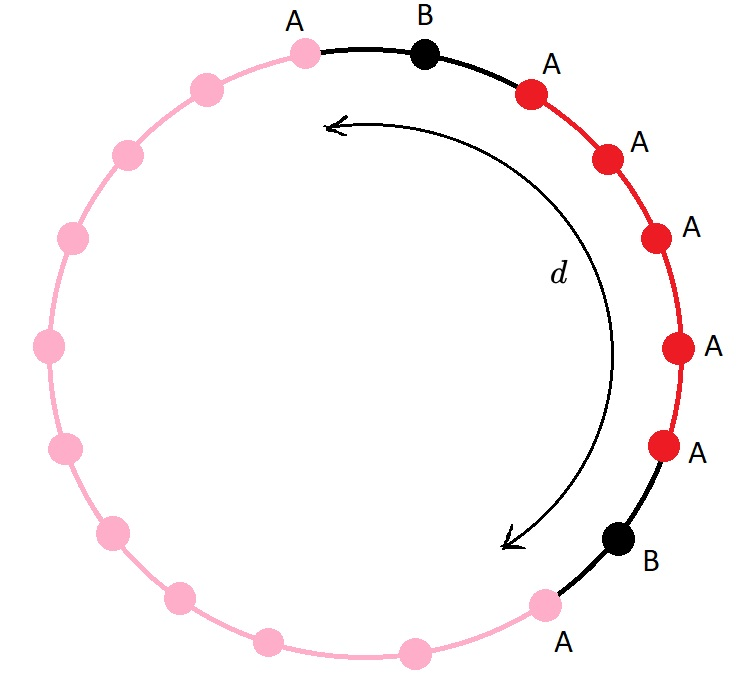
\includegraphics[width=0.4\textwidth]{figures/arc increase.jpg}
    \caption{}
\end{figure}

\begin{equation}
\begin{split}
    t_c &= \left[p^{k+1} \right] \times 0 \\
    &+ \left[ p^k\left( 1-p \right) \right] \times \left( t_{c-1} + t_{c+1} \right) \\
    &+ \left[1 - p^{k+1} - 2p^k\left( 1-p \right) \right] \times t_c \\
    &+ 1, \quad c \in \left\{ 2, 3, \hdots, d - k - 1 \right\}
\end{split}
\end{equation}
and following initial conditions:
\begin{equation}
\begin{split}
    t_1 &= \left[p^k\left( 1-p \right) \right] \times t_2 \\
    &+ \left[ 1 - p^k\left( 1-p \right) \right] \times t_1 \\
    &+ 1, \\
    t_{d-k-1} &= t_1
\end{split}
\end{equation}



\end{document}